This chapter presents the development process and details of the chosen GNU Radio applications for this thesis. \autoref{sect:gnu_radio_hack_rf_one_rtl_sdr_overview} provides an introduction to GNU Radio platform and application development, and the hardware later used for real-time testing (the HackRF One and the RTL-SDR). The following sections describe the two applications. The first, a WBFM Receiver, is intended as an introduction to developing SDR applications in GNU Radio and to demonstrate the potential for SDR to easily replace legacy analogue systems. The second, a PSK transceiver, will make full use of the SKSDR library and is intended to demonstrate application of several DSP blocks needed for digital communication systems.

%%%%%%%%%%%%%%%%%%%%%%%%%%%%%%%%%%%%%%%%%%%%%%%%%%%%%%%%%%%%%%%%%%%%%%%%%%%%%%%
\section{GNU Radio, HackRF One and RTL-SDR Overview}
\label{sect:gnu_radio_hack_rf_one_rtl_sdr_overview}

As previously mentioned, the hardware supporting this thesis is a HackRF One and an RTL-SDR. The HackRF One (shown in \autoref{fig:hackrf_one_detail}) is based on an analogue quadrature system, similar to the one described in \autoref{sect:analogue_quadrature_receiver_architecture}. The IF frequency is tuneable and is in 2.4 GHz industrial, scientific and medica (ISM) band. A high IF allows for a fairly relaxed image rejection filter. At the same time, it's relatively affordable to source IF mixer and VCO ICs designed to operate in the ISM bands. For critical phase noise and frequency stability (for example GPS applications) it's possible to install an external temperature compensated crystal oscillator (TCXO), which provide down to 0.5 ppm accuracy. Given the open hardware nature of this device, quite a few clones exist on the market. For this project, due to budget restrictions, a device sourced by Banggood was selected (specifically \href{https://pt.banggood.com/HackRF-One-1MHz-6GHz-Radio-Platform-Development-Board-Software-Defined-RTL-SDR-Demoboard-Kit-Dongle-Receiver-Ham-Radio-p-1552853.html}{this one})

\begin{figure} [ht]
  \begin{subfigure}{.5\textwidth}
    \centering
    \includegraphics[width=.8\linewidth]{hack_rf_one}
    \label{fig:hackrf_one_case}
  \end{subfigure}
  \begin{subfigure}{.5\textwidth}
    \centering
    \includegraphics[width=.8\linewidth]{hackrf_block_diagram}
    \label{fig:hackrf_one_block_diagram}
  \end{subfigure}
  \caption[The HackRF One case and block diagram]{The HackRF One comes with a brushed aluminium case and has 3 SMA ports (RF, Clock In and Clock Out). It has a 30 MHz to 6 GHz frequency range and 20 MHz bandwidth with 8 bits resolution [\citeauthor{hackrf_one_product}].}
  \label{fig:hackrf_one_detail}
\end{figure}

The RTL-SDR's original function is a DVB-T receiver but it was discovered by the community that it actually allows direct access to the IQ samples (in addition to the fully decoded MPEG signal which is its original application). This `undocumented' interface, however, has a limited bandwidth of 3.2 MHz. \autoref{fig:rtlsdr_detail} shows the physical format of the RTL-SDR USB dongle and a block diagram of its architecture. The device is based on a two-chip solution. An RF front-end (the R820T tuner IC) and the baseband IC composed of an ADC, video decoding and USB streaming logic. Note this IC is protected by non-disclosure agreement (NDA) so there is limited available knowledge about it.

\begin{figure} [ht]
  \begin{subfigure}{.5\textwidth}
    \centering
    \includegraphics[width=.6\linewidth]{rtlsdr_case}
    \label{fig:rtlsdr_case}
  \end{subfigure}
  \begin{subfigure}{.5\textwidth}
    \centering
    \includegraphics[width=1\linewidth]{rtlsdr_block_diagram}
    \label{fig:rtlsdr_block_diagram}
  \end{subfigure}
  \caption{The RTL-SDR USB dongle and the high-level block diagram, based on a two-chip solution [\citeauthor{rtlsdr_product}]}
  \label{fig:rtlsdr_detail}
\end{figure}

The applications are developed using the GNU Radio framework. GNU Radio is a free software development toolkit that provides signal processing blocks to implement software-defined radios and signal processing systems \cite{gnuradio_project}. It can be used with external RF hardware to create software-defined radios, or without hardware in a simulation-like environment. The GNU Radio applications consist of \emph{flowgraphs}, which are a series of connected signal processing blocks, thus describing a signal flow. The GNU Radio infrastructure is written entirely in C++, and many of the user tools are written in Python. Its graphical interface is supported by the Qt library (which as bindings for several languages such as Python through PyQt) and the wxWidgets library (considered deprecated for GNU Radio development, so its use is discouraged). GNU Radio runs mostly in GPP-based hardware although there are ongoing efforts to adapt the framework for FPGA and GPU-based platforms \cite{gr2020_program}.
\autoref{fig:simple_gr_demo} shows a very simple example of a flowgraph where one can see several types of blocks, like \emph{Source} and \emph{Sink}. Also, \emph{Variable} and \emph{Options} blocks, which allow for a more flexible workflow. Note that it's possible to use Python expressions and variables in most blocks input fields. The \emph{Throttle} block is usually used when there is no hardware limiting the sample rate, and its purpose is to prevent GNU Radio consuming samples as fast as possible, thereby consuming all the CPU time. In \autoref{fig:simple_gr_demo_exec} the \emph{Time Sink} interface is displayed, when the flowgraph is running. The frequency can be changed in real-time.

\begin{figure}[H]
  \centering
  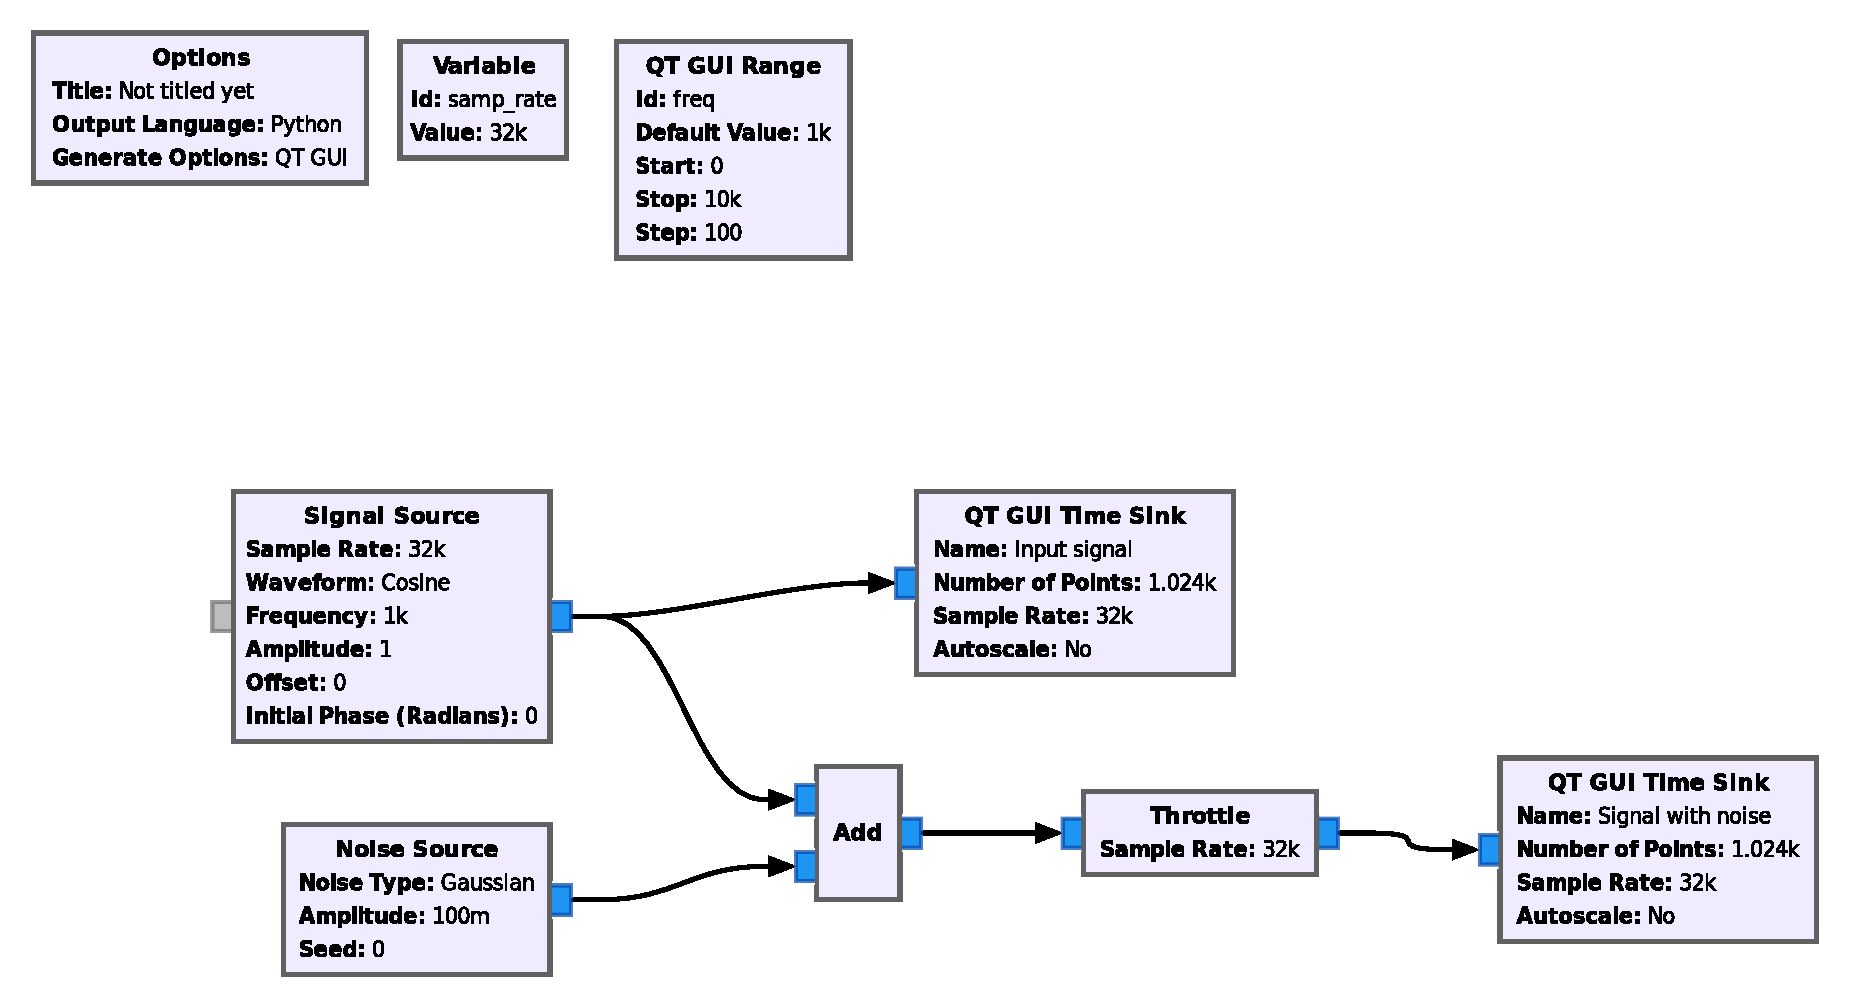
\includegraphics[width=0.75\textwidth]{simple_gr_demo}
  \caption[Simple GNU Radio flowgraph consisting of an input signal with added AWGN noise]{Simple GNU Radio flowgraph consisting of an input signal with added AWGN noise. The input signal with and without noise is visualized in a two \emph{Time Sink} blocks.}
  \label{fig:simple_gr_demo}
\end{figure}

\begin{figure}[H]
  \centering
  \includegraphics[width=0.75\textwidth]{simple_gr_demo_exec}
  \caption[Execution console for the flowgraph in \autoref{fig:simple_gr_demo}]{Execution console for the flowgraph in \autoref{fig:simple_gr_demo}. In GNU Radio it is possible to observe signals in real-time and to change simulation parameters, like the frequency in this case.}
  \label{fig:simple_gr_demo_exec}
\end{figure}

These flowgraphs are developed in GNU Radio Companion (GRC) (the graphical tool that comes with GNU Radio). This tool reads and writes files with .grc extension which are XML files (or YAML starting with GNU Radio 3.8) describing how the blocks are initialized and inter-connected (this is just for graphical rendering purposes). It also generates a Python file (usually with the same name) that has the actual Python code for creation of blocks, connections and all the glue code. This Python file can then be executed directly in GRC or in a terminal, and it will instantiate the workflow and pass it to the GNU Radio scheduler for execution. To be used in GRC, each block must also have a corresponding XML file that exposes its properties and that is read by GRC to render the block.
GNU Radio supports other advanced features such as tagged streams (for PDU oriented stream processing) and asynchronous message passing between blocks.

%%%%%%%%%%%%%%%%%%%%%%%%%%%%%%%%%%%%%%%%%%%%%%%%%%%%%%%%%%%%%%%%%%%%%%%%%%%%%%%
\section{WBFM Receiver with alternate algorithm}
\label{sect:WBFM_Receiver_with_alternate_algorithm}
Wideband (200 kHz) FM (WBFM) demodulation is an interesting use case that illustrates how SDR can replace legacy analogue systems with relative ease. \autoref{fig:wbfm_spectrum} shows the baseband spectrum of a typical FM radio signal.

\begin{figure}[H]
  \centering
  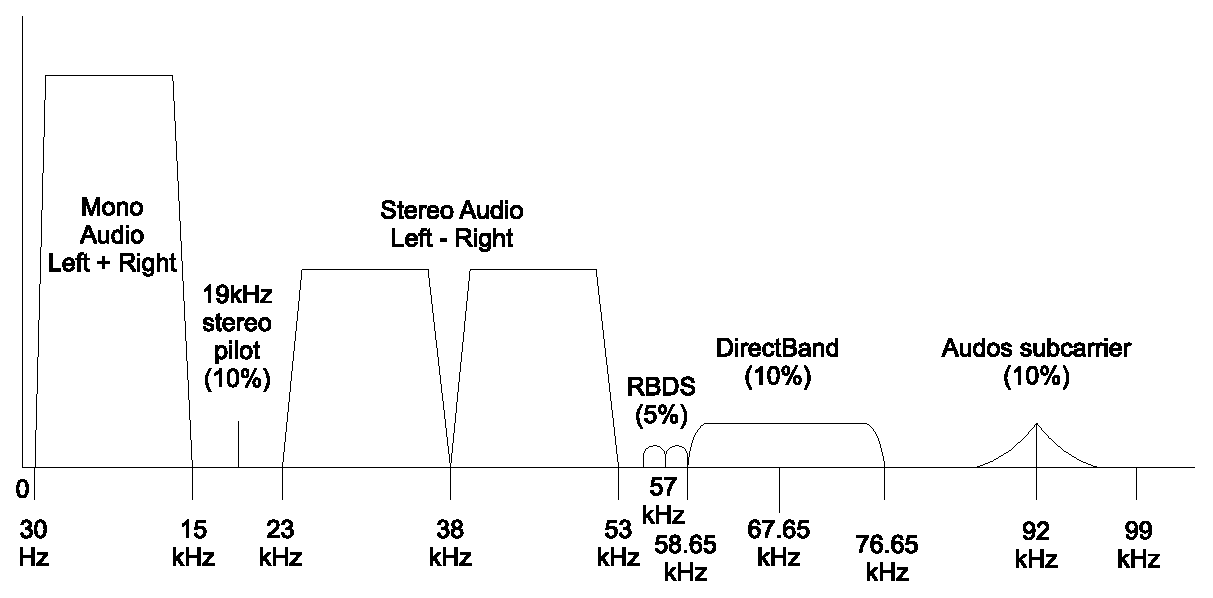
\includegraphics[width=0.75\textwidth]{wbfm_spectrum}
  \caption{Typical FM baseband spectrum, showing the different multiplexed services [\citeauthor{image:fm_spectrum}]}
  \label{fig:wbfm_spectrum}
\end{figure}

The main specifications of a classic FM broadcast system are as follows \cite{fm_demod2}:
\begin{itemize}
  \item Bandwidth: $\pm$75 kHz.
  \item Channel separation: 200 kHz.
  \item Mono channel is the algebraic sum of the left and right channels (L+R).
  \item Stereo channel is the algebraic difference of the left and right channels (L-R).
  \item Uses double-sideband suppressed-carrier (DSB-SC) modulation on the 38 kHz sub-carrier.
  \item Radio Data Services (RDS) is a communications protocol standard for embedding small amounts of digital information in conventional FM radio broadcasts. RDS standardizes several types of information transmitted, including time, station identification and program information. It uses BPSK digital modulation on the 57 kHz sub-carrier.
  \item 19 kHz pilot to assist in carrier recovery for Stereo and RDS demodulation.
  \item Other services on higher sub-carriers are part of the American Subsidiary Communications Authority (SCA) services.
\end{itemize}

The (L+R) main channel signal is transmitted as baseband audio limited to the range of 30 Hz to 15 kHz. The (L-R) signal is amplitude modulated onto a DSB-SC 38 kHz signal occupying the baseband range of 23 to 53 kHz. A 19 kHz pilot tone is also generated, which is used by the receiver to identify a stereo transmission and to regenerate the 38 kHz sub-carrier with the correct phase (usually using a PLL with a divider in the feedback path). Note this phase relationship is essential to reduce cross-talk between mono and stereo channels. The final multiplexed signal modulates the FM transmitter, with the deviation of the transmitter carrier frequency due to the stereo audio and pilot tone (at 10\% modulation) given by \cite{fm_demod}:
\begin{equation} \label{eq:fm_signal_freq}
  f_\Delta = \left(0.9\left(\frac{L+R}{2}+\frac{L-R}{2}\sin(4\pi f_p)\right)+0.1\sin(2\pi f_p)\right)\cdot 75 \text{ kHz}
\end{equation}
where $f_p$ is the frequency of the pilot tone (19 kHz).

\autoref{fig:fm_stereo_receiver} shows the block diagram of a stereo FM receiver. This particular two channel arrangement ensures compatibility with older mono-only receivers. On a stereo receiver, the main and secondary channels are added for the left side (producing $L+R+L-R=2L$ and hence eliminating the right side signal), and subtracted for the right side (producing $L+R-L+R=2R$ and hence eliminating the left side signal). Notice mono receivers still work since they only see the main channel which contains the combined audio signal (L+R).

\begin{figure}[H]
  \centering
  \includegraphics[width=0.75\textwidth]{fm_stereo_receiver}
  \caption{FM stereo block diagram [\citeauthor{HOOD199857}]}
  \label{fig:fm_stereo_receiver}
\end{figure}

GNU Radio already has a block that performs the necessary steps for FM demodulation (called \emph{WBFM Receive}) \cite{gnuradio_wbfm_receiver}. This block not only performs demodulation, but also high frequency de-emphasis needed for a typical FM broadcast system. One of the particularities is the use of the 4-quadrant arctangent function (\code{atan2()}), to compute the phase, which can prove difficult to implement, for example in some embedded systems. In reality, the function adopts a lookup table of 256 entries and makes other optimizations such as the $sin(x) \approx x$ approximation, in order to overcome this problem. However, as a way of exploring the capabilities of creating new blocks and extending the platform's functionality, an alternative algorithm was implemented (without using \code{atan2()}) based on the work of [\citeauthor{lyons2004}] \cite{wbfm_alt_receiver}. Details and comparison of the two demodulation techniques are presented in \autoref{sect:fm_demodulation}.

\autoref{fig:gr_tutorial_broadcast_fm_rx} shows a simple WBFM demodulator using a GNU Radio Companion flowgraph.
\begin{figure}[H]
  \centering
  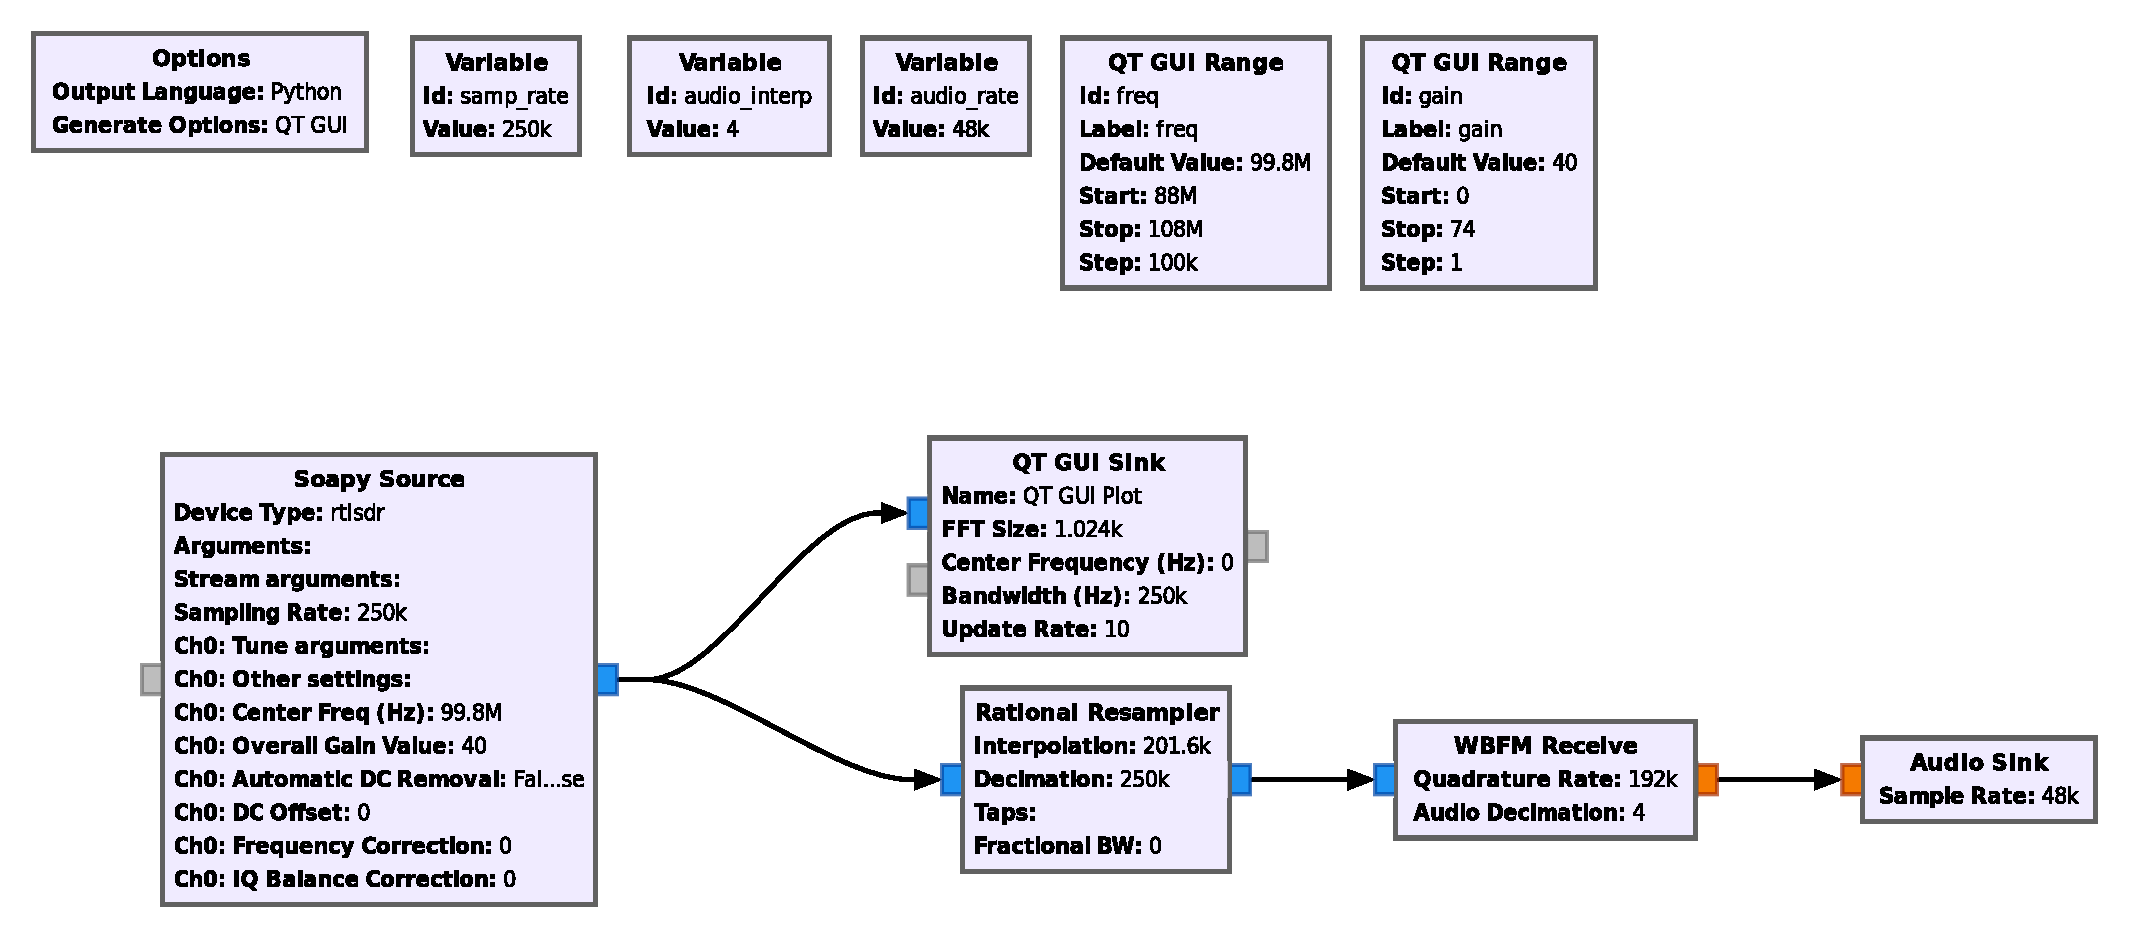
\includegraphics[width=\textwidth]{gr_tutorial_broadcast_fm_rx}
  \caption{FM demodulator using GNU Radio}
  \label{fig:gr_tutorial_broadcast_fm_rx}
\end{figure}
The \emph{Soapy Source} source block is a generic wrapper around SDR receivers. It supports many different hardware devices like the USRP, Airspy and RTL-SDR. When configured for RTL-SDR, it uses \code{librtlsdr}, which in turn configures and starts up the receiver, and collects the baseband IQ samples, via USB. The IQ stream is obtained in real time from the SDR and passes through a \emph{Rational Resampler} block that lowers the sample rate. The heart of the process is the \emph{WBFM Receive}. This block receives the IQ samples from the RTL-SDR receiver, demodulates de FM signal (only the mono channel) and streams the audio to an \emph{Audio Sink} or to a \emph{WAV File Sink}. GNU Radio also includes blocks to decode other services (for example \emph{GR-RDS} for RDS decoding). This demodulator works very well but is a black box so a more detailed description of the necessary steps to demodulate the signal is presented next. Note that some of these steps are optional (namely frequency shift to the desired station and multiple decimation steps), depending on how the RTL-SDR receiver's centre frequency and sampling rate are configured.

\subsection{IQ capture}

In order to focus on each individual step it's preferable to work with previously captured IQ samples instead of jumping immediately to a real-time system. Besides providing very useful GNU Radio blocks, Osmocom also maintain a collection of command line tools for testing the RTL-SDR, including collecting IQ samples, among other tasks. The tool is shown in \autoref{lst:rtlsdr_iq_recorder_syntax}.
\begin{bash}[label={lst:rtlsdr_iq_recorder_syntax},caption={RTL-SDR IQ recorder syntax}]
rtl_sdr, an IQ recorder for RTL2832 based DVB-T receivers

Usage: -f frequency_to_tune_to [Hz]
	[-s samplerate (default: 2048000 Hz)]
	[-d device_index (default: 0)]
	[-g gain (default: 0 for auto)]
	[-p ppm_error (default: 0)]
	[-b output_block_size (default: 16 * 16384)]
	[-n number of samples to read (default: 0, infinite)]
	[-S force sync output (default: async)]
	filename (a '-' dumps samples to stdout)
\end{bash}

For this example, 'Radio Comercial' station was chosen which broadcasts at 99.8 MHz with a 10 kW signal power from the Montejunto transmitter. A one second capture was performed with a sampling rate of 2.5 Msps and with a 40 RF dB gain applied. The command line used is shown in \autoref{lst:rtlsdr_iq_recorder_example}.

\begin{bash}[label={lst:rtlsdr_iq_recorder_example},caption={RTL-SDR IQ recorder example}]
rtl_sdr -f 99800000 -g 40 -s 2500000 -n 25000000 fm_iq_99.8MHz_2500kHz.dat

Found 1 device(s):
  0:  Realtek, RTL2838UHIDIR, SN: 00000001

Using device 0: Generic RTL2832U OEM
Found Rafael Micro R820T tuner
Exact sample rate is: 2500000.107620 Hz
[R82XX] PLL not locked!
Sampling at 2500000 S/s.
Tuned to 99800000 Hz.
Tuner gain set to 40.20 dB.
Reading samples in async mode...

User cancel, exiting...
\end{bash}

\subsection{Frequency Shifting}

If the channel of interest is not in the centre of the band then an initial frequency shift can be performed. Assume the wanted station is 99.8 MHz but the centre frequency was set to 100 MHz. The following complex multiplication can shift the station to the centre of the bandwidth:
\begin{equation} \label{eq:fm_signal_shift}
  x_{out}(n) = x_{in}(n)e^{-j(\omega_1 - \omega_0)n}
\end{equation}
where $\omega_1=100$ MHz and $\omega_0=99.8$ MHz in this case.

This is the well know result that a multiplication of two signals in time corresponds to convolving their spectra. Since the spectrum of the complex exponential is a frequency-shifted Dirac, this equates to shifting the spectrum of the input signal. Here one can start to appreciate the power of processing the signal in the digital domain. The analogue equivalent operation would require either a hardware mixer or at the very least some form of oscillator to generate the real and imaginary parts of the complex exponential and a multiplying block. In this case the RTL-SDR RF frequency was set to the desired station so there is no need for this frequency shift step.

\subsection{Decimation}

The next step that might be needed is to adjust the sampling rate to filter other stations and reduce the computational effort. The IQ capture was performed at much higher rate than is needed, since the station itself only occupies 75 kHz. This is shown in \autoref{fig:fm_iq_capture_plot_downshifted}, where the full 2.5 MHz bandwidth is visible, including the desired station and several others.

An initial decimation by 8 will bring the sampling rate to 312.5 kHz which is reasonable and allows for a second decimation at a later stage, to bring it down to an audio card sampling range. This decimation is usually preceded by a low pass filter to guard against aliasing. \autoref{fig:fm_iq_capture_plot_decimated8} shows the spectrum of the decimated signal with a new bandwidth of 312.5 kHz.

\begin{figure} [H]
  \begin{subfigure}{.5\textwidth}
    \centering
    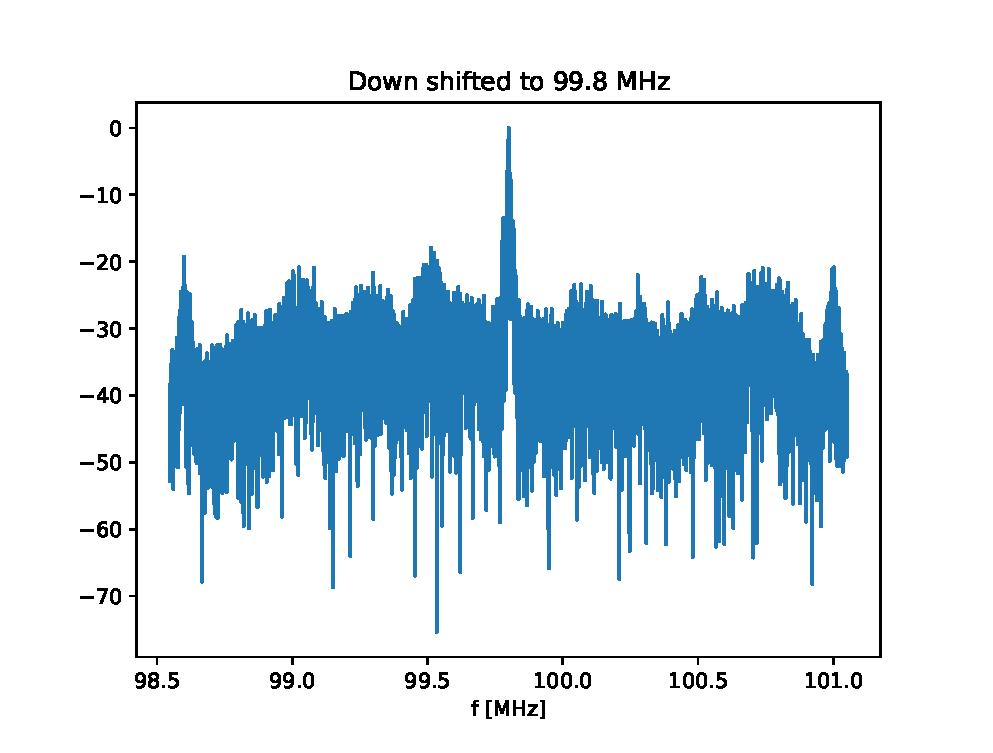
\includegraphics[width=\linewidth]{fm_iq_capture_plot_downshifted}
    \caption{Spectrum before decimation with a total bandwidth of 2.5 MHz}
    \label{fig:fm_iq_capture_plot_downshifted}
  \end{subfigure}%
  \begin{subfigure}{.5\textwidth}
    \centering
    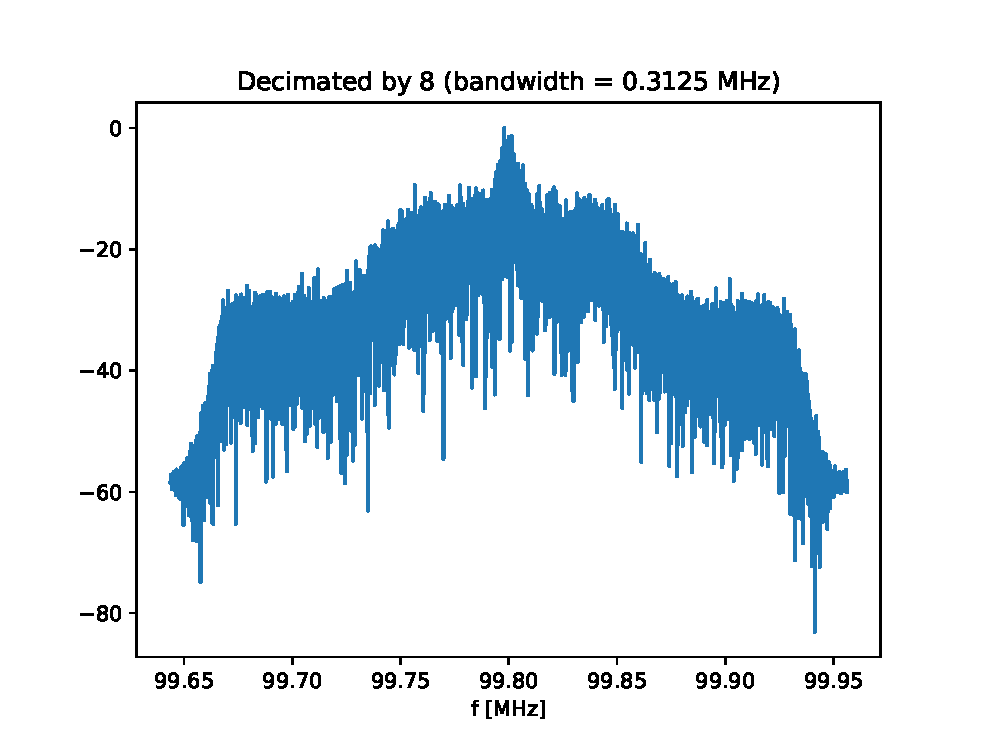
\includegraphics[width=\linewidth]{fm_iq_capture_plot_decimated8}
    \caption{Spectrum after decimation by 8, with a total bandwidth of 312.5 kHz}
    \label{fig:fm_iq_capture_plot_decimated8}
  \end{subfigure}
  \caption{Complex IQ baseband spectrum of input signal, before and after decimation}
\end{figure}

\subsection{Demodulation} \label{sect:fm_demodulation}

The final stage is the actual demodulation of the FM signal. There are perhaps as many techniques for frequency detection as there are designers who have considered the problem. Despite this, they usually fall within the following four categories \cite{communication_systems_carlson}:
\begin{enumerate}
  \item FM-to-AM conversion
  \item Phase-shift discrimination
  \item Zero-crossing detection (not discussed in this thesis)
  \item Frequency feedback (PLL based detection, also not discussed in this thesis)
\end{enumerate}

GNU Radio's demodulator is based on technique 2. The underlying principle comes from an approximation for time differentiation:
\begin{equation}
  \dot{\upsilon}(t) \approx \frac{1}{\Delta t}\left(\upsilon(t) - \upsilon\left(t-\Delta t\right)\right)
\end{equation}

provided $\Delta t$ is small compared to the variation of $\upsilon(t)$. An FM signal has $\dot\phi (t)=2\pi f_{\Delta} x(t)$ (where $\dot\phi$ denotes differentiation with respect to time), so by applying this technique, one gets
\begin{equation}
  \phi(t) - \phi(t-\Delta t) \approx \Delta t \dot\phi(t) = \Delta t 2\pi f_{\Delta} x(t)
\end{equation}
and so it's possible to obtain an approximation to the signal's frequency by the phase difference between two consecutive samples. As mentioned, however, to obtain this phase difference requires an arctangent operation.

The proposed alternative in this thesis falls within the scope of technique 1, although with a variation. The classical FM-to-AM conversion works on the principle that it's possible to extract the frequency of a sinusoidal signal by differentiation. Let $x_c(t)=A_c \cos(\theta{_c}t)$ with $\dot\theta_c(t)=2\pi\left(f_c+f_{\Delta}x(t)\right)$, then
\begin{equation} \label{eq:fm_signal}
  \dot{x}_c(t) = -A_c\dot\theta_c(t) \sin(\theta{_c}t)
\end{equation}

Hence an envelope detector with input $\dot{x}_c(t)$ yields an output proportional to $f(t) = f_c+f_{\Delta}x(t)$. Instead of 'extracting' the argument of the sinusoid by differentiating the entire signal, an alternative is to differentiate just the instantaneous phase (the argument of the sinusoid), provided there is a way to obtain this instantaneous phase. This approach is depicted in \autoref{fig:wbfm_atan}.

\begin{figure}[H]
  \centering
  \includegraphics[width=\textwidth]{wbfm_atan}
  \caption{Frequency demodulator using an arctangent function [\citeauthor{wbfm_alt_receiver}]}
  \label{fig:wbfm_atan}
\end{figure}

The demodulator's instantaneous output frequency is
\begin{equation} \label{eq:digital_fm_demod}
  f(n)= \frac{f_s}{2\pi}\Delta\theta(n)
\end{equation}
where $f_s$ is the sampling frequency in Hz.

Computing instantaneous phase $\theta(n)$, again, requires an arctangent operation, which could difficult to implement accurately without considerable computational resources. Only this time there is an alternative. The following algorithm computes $\Delta\theta(n)$ for use in expression \eqref{eq:digital_fm_demod}, without the intermediate $\theta(n)$ phase computation. Given the following definitions:
\begin{itemize}
  \item $i(t)$ = in-phase signal
  \item $q(t)$ = quadrature phase signal
  \item $r(t)=q(t)/i(t)$
  \item $\theta(t) = tan^{-1}\left(\frac{q(t)}{i(t)}\right)$ = instantaneous phase
  \item $\Delta\theta(t)$ = time derivative of $\theta(t)$
\end{itemize}

The time derivative of $\tan^{-1}(r(t))$ is
\begin{equation} \label{eq:fm_no_atan_1}
  \Delta\theta(t) = \diff{(\tan^{-1}(r(t)))}{t}=\frac{1}{1+r^2(t)}\diff{r(t)}{t}
\end{equation}

knowing that $\diff{r(t)}{t}=\diff{(q(t)/i(t))}{t}$, then
\begin{equation} \label{eq:fm_no_atan_2}
  \diff{r(t)}{t} = \diff{(q(t)/i(t))}{t} = \frac{i(t)\diff{q(t)}{t}-q(t)\diff{i(t)}{t}}{i^2(t)}
\end{equation}

Plugging \eqref{eq:fm_no_atan_2} result into \eqref{eq:fm_no_atan_1}, yields
\begin{equation} \label{eq:fm_no_atan_3}
  \Delta\theta(t) = \diff{(\tan^{-1}(r(t)))}{t}=\frac{1}{1+r^2(t)}\frac{i(t)\diff{q(t)}{t}-q(n)\diff{i(t)}{t}}{i^2(t)}
\end{equation}

Finally, the numerator and denominator of the first ratio in \eqref{eq:fm_no_atan_3} are multiplied by $i^2(t)$, and the discrete time variable index $n$ replaces $t$, to arrive at the result of
\begin{equation} \label{eq:fm_no_atan_4}
    \Delta\theta(n)= \frac{i(n)\diff{q(n)}{n}-q(n)\diff{i(n)}{n}}{i^2(n)+q^2(n)}
\end{equation}

The implementation of this algorithm, where the derivatives of $i(n)$ and $q(n)$ are $i'(n)$ and $q'(n)$ respectively, is shown in \autoref{fig:wbfm_no_atan}.

\begin{figure}[H]
  \centering
  \includegraphics[width=\textwidth]{wbfm_no_atan}
  \caption{Frequency demodulator without arctangent: (a) standard process; (b) simplified process [\citeauthor{wbfm_alt_receiver}]}
  \label{fig:wbfm_no_atan}
\end{figure}

The $\Delta\theta(n)$ output sequence is used in \eqref{eq:digital_fm_demod} to compute instantaneous frequency. The Differentiator is a FIR differentiating filter with an odd number of taps. The Delay elements are needed to time-align $i(n)$ and $q(n)$ with the outputs of the differentiators such that the delay is $(K-1)/2$ samples when a K-tap differentiator is used. A simplified version of this algorithm (shown in \autoref{fig:wbfm_no_atan} b)) can be used, if the signal is purely FM and hard limited such that $i^2(n)+q^2(n)=k$ (where k is constant), and using [1, 0, -1]-coefficient differentiators.

The resulting spectrum from the demodulation is shown in \autoref{fig:fm_iq_capture_plot_demodulated}. The last step is to decimate once more to bring the signal into the sampling range of the audio card, while filtering everything above the mono channel. Using a decimation by 10 results in the spectrum shown in \autoref{fig:fm_iq_capture_plot_decimated10} with a final bandwidth of 31.25 kHz.

\begin{figure} [H]
  \begin{subfigure}{.5\textwidth}
    \centering
    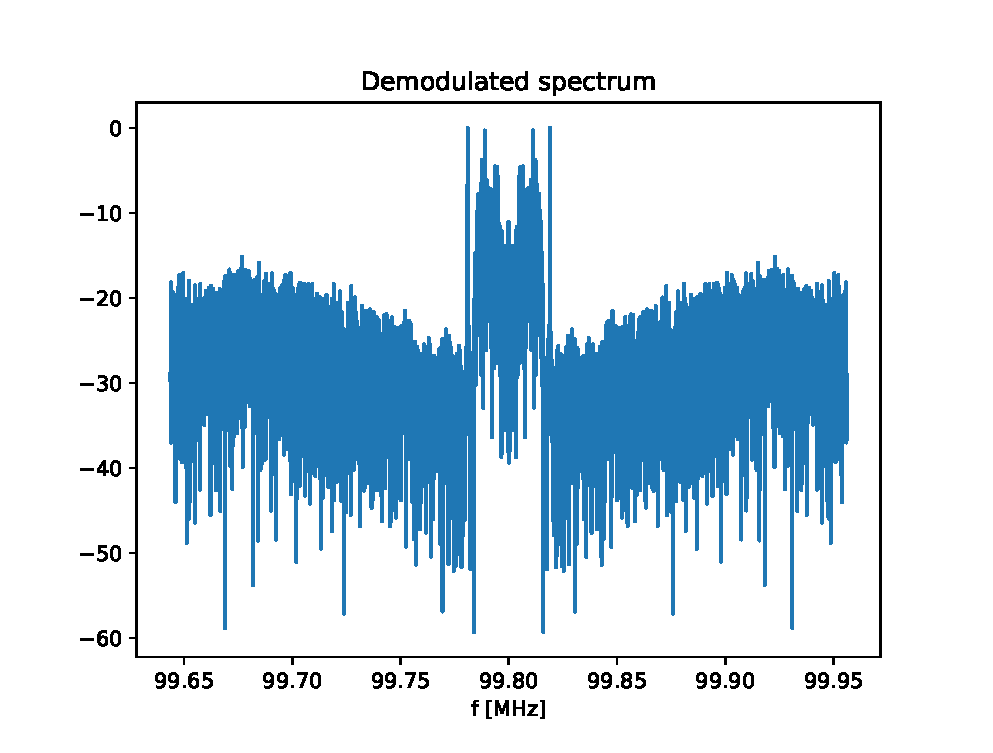
\includegraphics[width=\textwidth]{fm_iq_capture_plot_demodulated}
    \caption{Spectrum of demodulated signal, before final decimation}
    \label{fig:fm_iq_capture_plot_demodulated}
  \end{subfigure}%
  \begin{subfigure}{.5\textwidth}
    \centering
    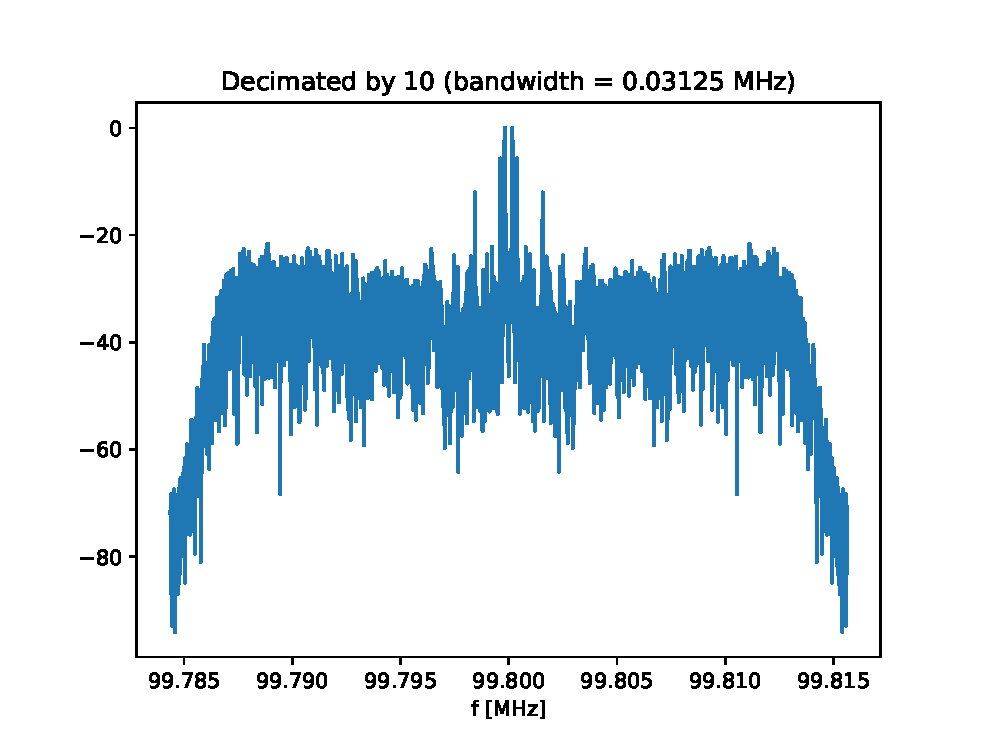
\includegraphics[width=\textwidth]{fm_iq_capture_plot_decimated10}
    \caption{Spectrum of demodulated signal, now decimated to 31.25 kHz}
    \label{fig:fm_iq_capture_plot_decimated10}
  \end{subfigure}
  \caption{Demodulated FM spectrum, before and after decimation}
\end{figure}

The demodulated signal is purely real. It is no longer a complex IQ signal. From a spectral point of view, this means the negative frequency side is a conjugate-mirror image of the positive frequency side. Comparing with the typical FM spectrum shown in \autoref{fig:wbfm_spectrum}, it's possible to clearly identify the mono audio channel (L+R), 19 kHz stereo pilot, stereo audio channel (L-R), and RDS signal.

\autoref{fig:wbfm_alt_receiver_gr_flowgraph} shows the developed GR alternative WBFM demodulator based on this algorithm. A prototype of the algorithm was built in Python with the differentiator filter design and coefficients generation made through the SciPy library. The result is in good agreement with the theory and demodulation is successful. This flowgraph is then housed in a hierarchical block (GNU Radio supports the concept of hierarchical blocks, which act containers for other blocks) and can be used as a drop-in replacement for the standard GR \emph{WBFM Receive}, for demodulation in real time.

\begin{figure}[H]
  \centering
  \includegraphics[width=\textwidth]{wbfm_alt_receiver_gr_flowgraph}
  \caption[Alternate WBFM receiver implementation as a GR hierarchical block]{Alternate WBFM receiver implementation as a GR hierarchical block. Notice the 15 samples delay, necessary to make the differentiating filter causal, shifting it by $(K-1)/2$ samples, with $K$ the number of taps of the filter, in this case 31.}
  \label{fig:wbfm_alt_receiver_gr_flowgraph}
\end{figure}

\autoref{fig:wbfm_alt_receiver_gr_exec} shows the execution, and spectrum of the FM signal after demodulation.

\begin{figure}[H]
  \centering
  \includegraphics[width=\textwidth]{wbfm_alt_receiver_gr_exec}
  \caption[Runtime interface for the alternate WBFM receiver]{Runtime interface for the alternate WBFM receiver, allowing also to set the frequency and IF gain. Besides the real demodulated spectrum, it is possible to observe the $\pm$ 19 kHz pilot sub-carrier.}
  \label{fig:wbfm_alt_receiver_gr_exec}
\end{figure}

\section{PSK Transceiver}
\label{sect:psk_transceiver}

The idea of this application is to develop a fully functional PSK transceiver using a GNU Radio flowgraph. The requirements include end-to-end transmission both in a propagated medium (a waveguide) and a radiated environment. The HackRF One will serve as the transmitter and the RTL-SDR as the receiver.

The specifications for this system are:
\begin{enumerate}
  \item Frame structure: 26 bit preamble (13 bit Barker sequence $\times$ 2) + 224 bit payload = 250 bits
  \item Modulation: BPSK and QPSK with $\text{amplitude}=1$ and
  \item Sampling frequency: 1.024 MHz
  \item Transmitter upsampling: 4
  \item Transmit filter: Square-root raised cosine (RRC)
  \item Receiver downsampling: 2
  \item Receiver filter: Matched filter (RRC)
  \item Gain control: AGC
  \item Synchronization: Carrier Frequency and Symbol Timing (using a ZCTED)
  \item Coding: Scrambling/Descrambling (needed for the ZCTED). Optional Hamming(7,4) FEC.
  \item Frame detection: Correlation-based
\end{enumerate}

The application takes full advantage of the algorithms already developed in the SKSDR library to solve the problems presented by a real life transceiver (as opposed to a simulation environment) such as carrier frequency synchronization, timing synchronization and signal amplitude control.
By encapsulating most of the logic in the library, the GR blocks can be developed as thin wrappers which speeds up development. \autoref{fig:psk_tx_mine} shows the transmitter flowgraph. Most of the blocks (the ones with entirely lower case title and underscores) are custom developed GR Python blocks that encapsulate the corresponding module in the SKSDR library. All of the transmitter settings can be parametrized through variables. In addition, all of the developed blocks (both in the library and GR) include logging facility that can be turned on/off via the \emph{Python Snippet} block. This is very useful for debugging.

\begin{sidewaysfigure}[ht]
  \centering
  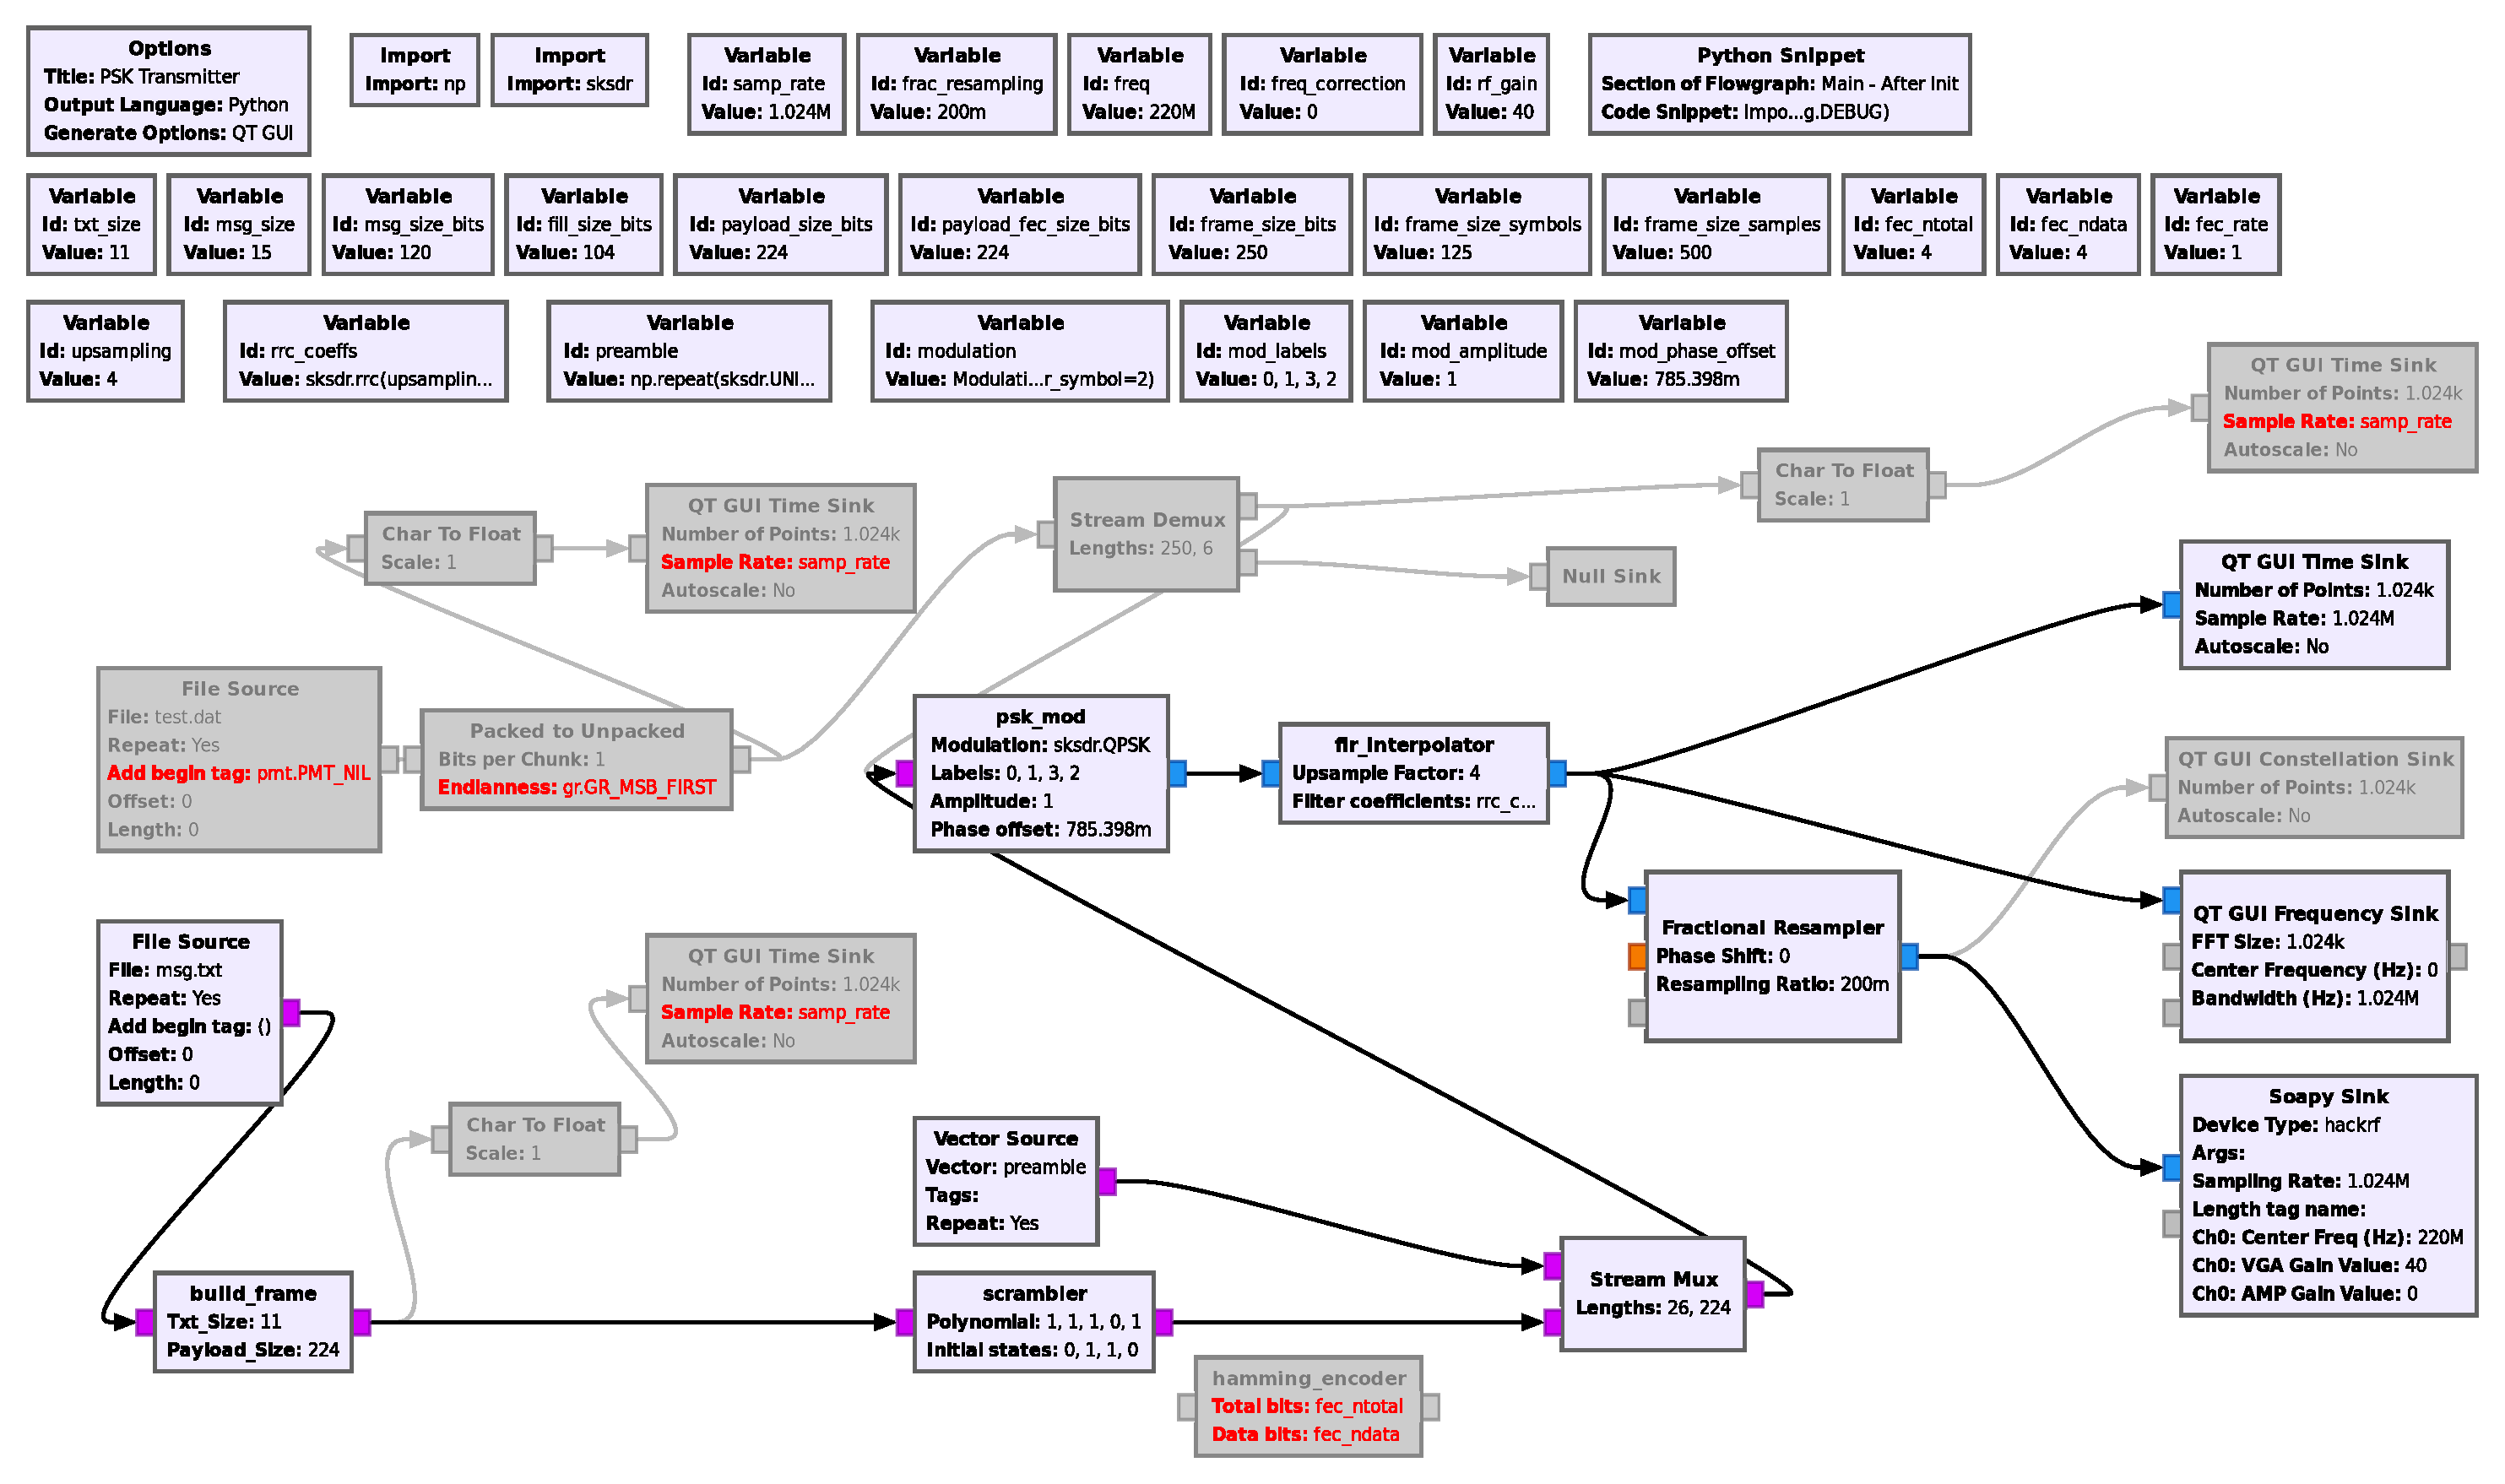
\includegraphics[width=\textwidth]{psk_tx_mine}
  \caption{PSK transmitter flowgraph}
  \label{fig:psk_tx_mine}
\end{sidewaysfigure}
\FloatBarrier
The \emph{File Source} block provides the text message to be sent, outputting it as 8-bit chars. The \emph{build\_frame} block takes these bytes, turns them into a bit stream and adds random padding to achieve the specified payload size. This payload is then passed to the \emph{scrambler} block for scrambling. After this, the preamble and payload are muxed together and sent to the PSK modulator (the \emph{psk\_mod} block). Finally, the symbols output by the modulator are upsampled by 4 and RRC filtered, before being sent to the HackRF. Note there is an additional block called \emph{Fractional Resampler} before the HackRF. This is because the HackRF minimum sample rate is 1 MHz (1.024 MHz was chosen as it is the minimum common for both transmitter and receiver) but the  modules developed are not capable of delivering that performance (chiefly because of being developed in Python). As such, to avoid the HackRF underflowing, a GR standard resampler (the \emph{Fractional Resampler}) is inserted before the HackRF. This block introduces an additional upsample (by a factor of 5) that overcomes this problem. \autoref{fig:psk_tx_mine_exec} shows the execution console for the transmitter, where the signal at the output of the \emph{fir\_interpolator} block can be observed.

\begin{figure}[H]
  \centering
  \includegraphics[width=\textwidth]{psk_tx_mine_exec}
  \caption{PSK transmitter execution showing the \emph{fir\_interpolator} block in time and frequency domains}
  \label{fig:psk_tx_mine_exec}
\end{figure}

The receiver flowgraph is shown in \autoref{fig:psk_rx}. The receiver starts by downsampling using the \emph{Fractional Resampler} to remove the additional upsampling introduced in the transmitter. The signal is then passed to the AGC for amplitude control. The AGC is configured to average over an entire frame. At this stage the signal is still upsampled by 4 and, given QPSK is being used, a 250 bit frame corresponds to 125 symbols (2 bits per symbol), which upsampled by 4 totals 500 samples. The signal is then decimated by 2 (\emph{fir\_decimator} block) and ready to go the synchronization stages. An initial frequency compensation is performed by the \emph{coarse\_freq\_comp} block and then carrier frequency synchronization is performed by the \emph{freq\_sync} block, followed by symbol timing synchronization (\emph{symbol\_sync} block). At this point the signal is just one sample per symbol. These samples are then passed to the \emph{frame\_sync} block, whose job is to find the beginning of a frame, by correlating the incoming samples stream with the known modulated preamble. If a valid frame is detected, then it is output and sent for demodulation. Note there is an additional block (\emph{phase\_offset\_est}) before the PSK demodulator. This block corrects possible mistakes from the synchronization stages, which can lock on to any of four different phases for QPSK, or two phases for BPSK (see \autoref{sect:library_freq_sync}). After this, the symbols are sent to the demodulator (\emph{psk\_demod} block). Finally the recovered bits are descrambled and sent to the \emph{decode\_frame} block which simply converts the unscrambled bits to their text representation. \autoref{fig:psk_rx_exec} shows the execution console for the receiver, where the signal at the output of the \emph{coarse\_freq\_comp} block can be observed.

\begin{sidewaysfigure}[ht]
  \centering
  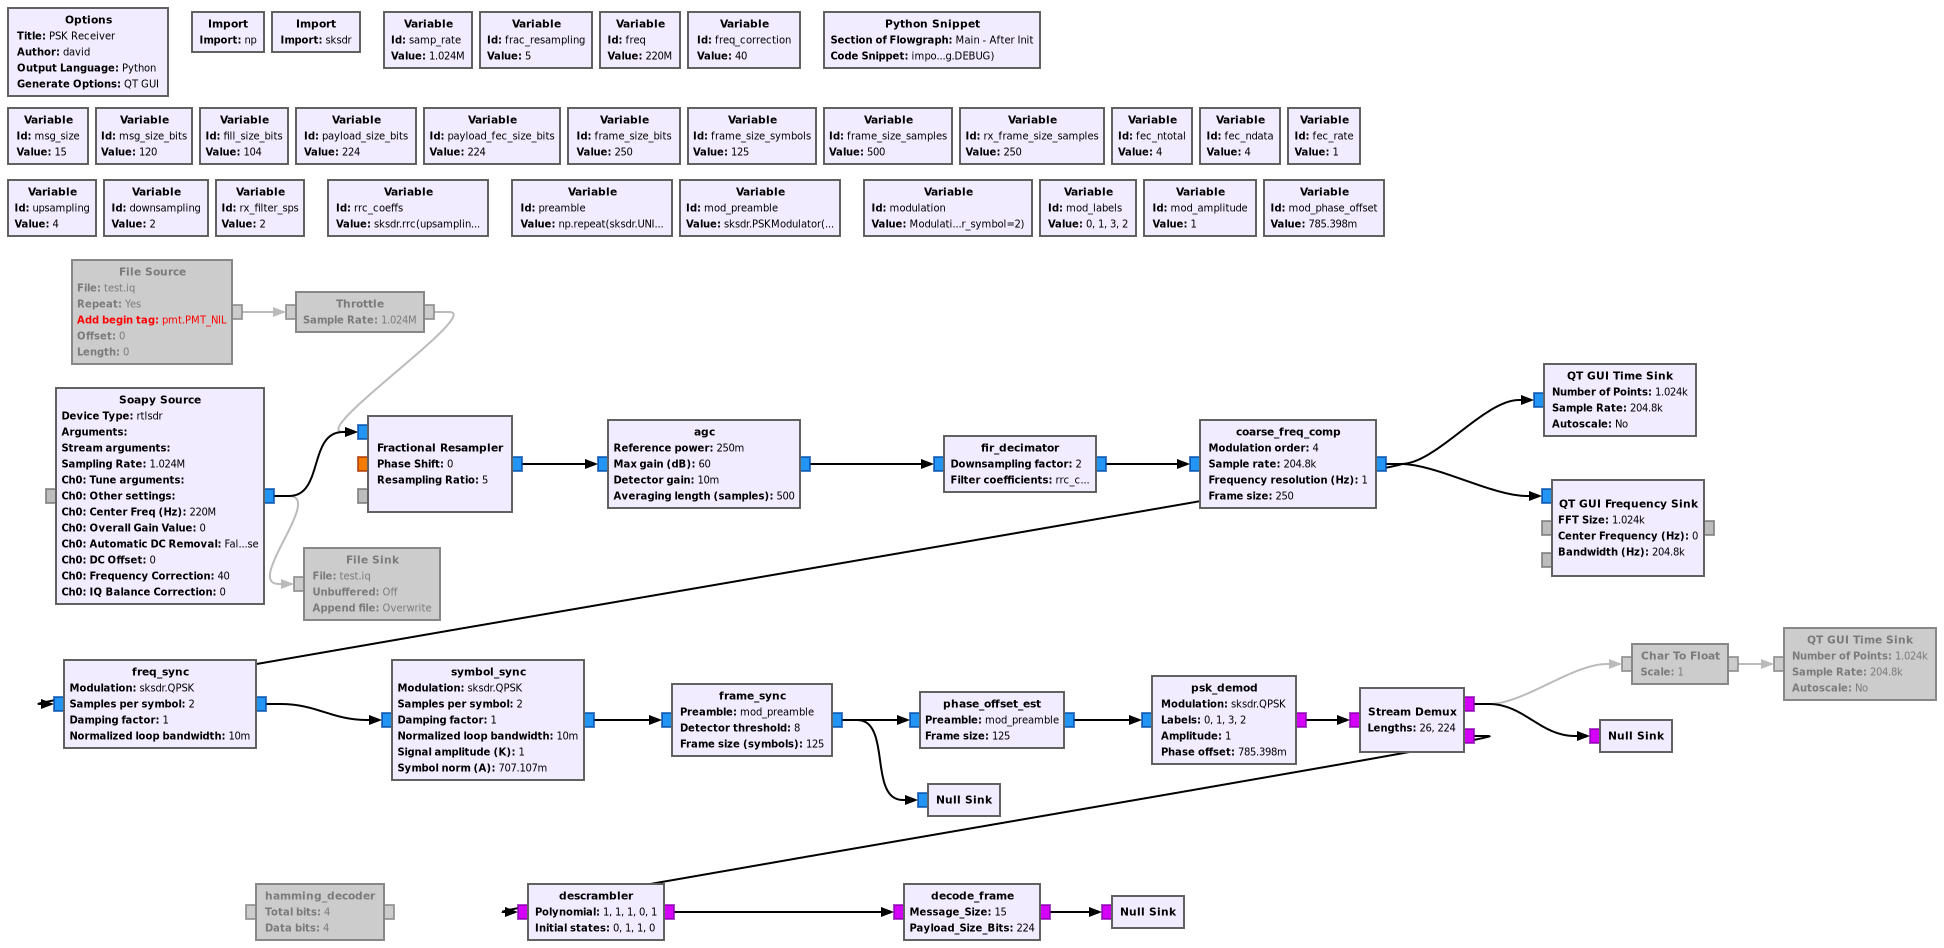
\includegraphics[width=\textwidth]{psk_rx2}
  \caption{PSK receiver flowgraph}
  \label{fig:psk_rx}
\end{sidewaysfigure}
\FloatBarrier
\begin{figure}[H]
  \centering
  \includegraphics[width=\textwidth]{psk_rx_exec}
  \caption{PSK receiver execution showing the output of the \emph{coarse\_freq\_comp} block in time and frequency domains}
  \label{fig:psk_rx_exec}
\end{figure}

\begin{figure}[H]
  \centering
  \includegraphics[width=\textwidth]{psk_rx_stream}
  \caption{PSK receiver terminal showing the correctly received frames being output by the \emph{decode\_frame} block}
  \label{fig:psk_rx_stream}
\end{figure}

In alternative to a real-time reception, one can send the output of the transmitter to a file, or collect the received IQ samples in a file, which can then be processed. To do this in the receiver flowgraph, one just needs to enable the \emph{File Sink} block to store the received samples (see the grey blocks in the flowgraph, which are disabled), and then process that same file, enabling in turn the \emph{File Source} block.

Yet another alternative in to use \code{PSKTrans} Python class in the SKSDR library, which also implements a PSK transceiver. This is a good option for initial stages of development, since the Python class execution can be inspected, traced using a debugger, which allows for an easier analysis of the input and outputs of each block, and the overall logic of the transceiver. \autoref{lst:psk_trans} shows the \code{PSKTrans} class constructor, which instantiates the transceiver with a reasonable set of default values, but allows one to specify any other values as well.

\begin{python}[label={lst:psk_trans},caption={\code{PSKTrans} class in the SKSDR library}]
class PSKTrans:
def __init__(self, sample_rate=200.0e3, upsampling=4, downsampling=2, frame_size=100,
  # Modulation
  modulation=QPSK, mod_symbols=[0, 1, 3, 2], mod_amplitude=1.0, mod_phase_offset=np.pi/4,
  # Scrambling
  scrambler_poly=[1, 1, 1, 0, 1], scrambler_init_state=[0, 1, 1, 0],
  # RRC filtering
  rrc_rolloff=0.5, rrc_span=10,
  # AGC agc_ref_power = 1/upsampling
  agc_ref_power=1/4, agc_max_gain=60.0, agc_det_gain=0.01, agc_avg_len=100,
  # Coarse frequency compensation
  coarse_freq_comp_res=25.0,
  # Frequency synchronization
  fsync_damp_factor=1.0, fsync_norm_loop_bw=0.01,
  # Symbol timing synchronization
  ssync_K=1.0, ssync_A=1/np.sqrt(2), ssync_damp_factor=1.0, ssync_norm_loop_bw=0.01,
  # Frame synchronization
  prb_det_thr=8.0,
  # Channel settings
  chan_snr=np.inf, chan_signal_power='measured',
  chan_delay_type='triangle', chan_delay_step=0.0, chan_max_delay=0.0,
  chan_freq_offset=0.0, chan_phase_offset=0.0):
\end{python}

\section{GNU Radio Stream Demux Module}
\label{sect:gr_stream_demux}

During the testing of the PSK transceiver of \autoref{sect:psk_transceiver} a block was needed that would separate the preamble from the payload (see \autoref{fig:psk_rx}). Since this block was not available in the GNU Radio codebase, a new C++ block named \emph{Stream Demux} was developed. This block, as the name implies, separates the input stream into a number of output streams, with each output stream having a distinct number of samples.

To develop new blocks, GNU Radio provides the out-of-tree (OOT) concept, which allows one to develop a new block outside of the main GNU Radio codebase, but install it locally side-by-side with GNU Radio. GR provides a tool called \code{gr\_modtool} that manages all the functionality of new modules, including a wizard to create the initial set of files. The code for this block is available at \cite{gr_stream_demux}. \autoref{lst:stream_demux} shows the \code{general\_work()} function which implements the main part of the block's logic.

\begin{cpp}[label={lst:stream_demux},caption={Stream Demux \code{general\_work()} function}]
int stream_demux_impl::general_work(int noutput_items,
                                gr_vector_int& ninput_items,
                                gr_vector_const_void_star &input_items,
                                gr_vector_void_star &output_items)
{
    char* out;
    const char* in = (const char*)input_items[0];
    int input_index = 0;                             // Items read
    gr_vector_int output_index(d_lengths.size(), 0); // Items written
    std::vector<gr::tag_t> stream_t;

    while (input_index < ninput_items[0]) {
        if (noutput_items <= output_index[d_stream]) {
            break;
        }
        int space_left_in_buffers = std::min(
            ninput_items[0] - input_index,         // Space left in input buffer
            noutput_items - output_index[d_stream] // Space left in output buffer
        );
        int items_to_copy = std::min(space_left_in_buffers, d_residual);
        in = (const char*)input_items[0] + input_index * d_itemsize;
        out = (char*)output_items[d_stream];
        memcpy(&out[output_index[d_stream] * d_itemsize], in, items_to_copy * d_itemsize);
        get_tags_in_window(stream_t,
                           0,
                           input_index,
                           input_index + items_to_copy);
        for (auto t : stream_t) {
             t.offset = t.offset - nitems_read(0) - input_index +
                        nitems_written(d_stream) + output_index[d_stream];
             add_item_tag(d_stream, t);
        }

        output_index[d_stream] += items_to_copy;
        input_index += items_to_copy;
        d_residual -= items_to_copy;
        if (d_residual == 0) {
            do { // Skip all those outputs with zero length
                d_stream = (d_stream + 1) % d_lengths.size();
            } while (d_lengths[d_stream] == 0);
            d_residual = d_lengths[d_stream];
        } else {
            break;
        }
    } // while

    consume(0, input_index);

    for (size_t i = 0; i < output_index.size(); i++) {
        produce((int)i, output_index[i]);
    }

    return WORK_CALLED_PRODUCE;
}
\end{cpp}

Since this block could be useful for others (there is an open feature request for this, GNU Radio issue \#1995), it was proposed to be integrated in GNU Radio's main codebase. For this to happen, however, quite a few other files need to be changed, like Makefiles, documentation and unit testing. The block was integrated on 25/09/2020 (see the \href{https://github.com/gnuradio/gnuradio/commit/c196dacea56ef938902646a2143907858415b240}{commit log}).
